%!TEX program = pdflatex
\documentclass[conference]{IEEEtran}
\usepackage{amssymb}
\usepackage{enumitem}
\usepackage{graphicx}
\graphicspath{{visualize/}}
\usepackage{epstopdf}
\usepackage{amsmath}
\usepackage{bbm}
\usepackage[footnotesize]{caption}
\usepackage{subcaption}
\usepackage{cite}
\usepackage{flushend}
\usepackage{xifthen}


\begin{document}
\title{BC Description and Visualization}
\maketitle

\section{Level Evaluation} \label{sec:LevelEvaluation}
We used Mario AI Framework to evaluate each level generated by the GAN. According to the AI agent's result, we assigned 
a fitness value $f$ to each level. We defined $f$ to be the percentage of completion, as Equation ~\ref{eqn:fitness}
shows:
\begin{equation}
    f=\frac{d_{completed}}{d_{level}}
    \label{eqn:fitness}
\end{equation}
where $d_{completed}$ was the distance that the AI agent went through and $d_{level}$ was the full distance of that level. 

To map the latent vector onto the elite map, we also extracted Behavioral Characteristics ($BC$s) from each level. These
$BC$s corresponded to the dimensions of the elite maps, and were either $static$ (could be observed before the AI 
agent played it), such as the number of enemies in a level, or $dynamic$ (were obtained from the AI agent's 
actions), such as whether the agent jumped while playing the level. We tried 3 sets of $BC$s as dimensions of 
our elite maps, and next we would discuss each set of $BC$s selected.

\subsection{Mario GAN $BC$s}
In this setting, We used two $BC$s to describe the "style" of a Mario level: the number of tiles in the sky and 
the number of enemies. Both of them were static and were observed before the AI agent started to play the level.

"Tiles in the sky" referred to all game objects (\textbf{i.e. }normal blocks, question blocks, coins) 
that could only be reached if Mario jumped. We assumed that a large value meant that there were many game elements 
above the ground and the player was encouraged jump to higher levels, while a small value implied that player would 
stay on the ground most of the time. 

"Number of enemies" was the number of enemies in the whole level. Our GAN could generate 4 types of enemies: 
Spiky, Goomba, Green Goomba and Red Goomba. We assumed that this value reflected the intenseness of a level. 
\subsection{8 Binary $BC$s}
This setting corresponded to the "Constrained Map-Elites’ dimensions" in previous work (Citaion Needed). We collected 8 
$BC$s according to the AI agent's actions while playing. In other words, all the 8 $BC$s were $dynamic$. In addition, each $BC$ was binary, representing whether the AI agent performed
the action or satisfied certain condition. In this way, our elite map had 8 binary dimensions and $2^8$ cells. Table 
\ref{tab:8BCs} described the 8 $BC$s we used. \\
\begin{table}[h!]
    \centering
    \begin{tabular} {|p{0.20\linewidth}|p{0.70\linewidth}|}
        \hline
        $BC$ & Description \\
        \hline \hline
        Jump & 1 if the agent jumped at least once in this level, 0 otherwise.\\
        \hline
        High Jump & 1 if the agent had stayed in air more than a certain amount of time during one jump (meaning that it travelled more than a certain distance vertically within one jump), 0 otherwise.\\
        \hline 
        Long Jump & 1 if the agent had travelled more than a certain distance horizontally within one jump, 0 otherwise.\\
        \hline
        Stomp Kill & 1 if the agent killed at least one enemy by stompping (jumped onto it from above), 0 otherwise.\\
        \hline
        Shell Kill & 1 if the agent killed at least one enemy using koopa shell, 0 otherwise.\\
        \hline
        Fall Kill & 1 if there was at least one enemy that was killed because of falling out of the map, 0 otherwise.\\
        \hline
        Mushroom & 1 if the agent collected at least one mushroom, 0 otherwise.\\
        \hline
        Coin & 1 if the agent collected at least one coin, 0 otherwise.\\
        \hline
    \end{tabular}
\caption{Descriptions of the 8 $BC$s used in the 8 Binary $BC$s setting.}
\label{tab:8BCs}
\end{table}
\subsection{KL Divergent $BC$s}
Under this setting, we selected two scenes from two different \textbf{original} Mario levels, as shown in Figure \ref{fig:KLDiv}. 
The two $BC$s of a newly generated level were given by its KL Divergent values with each of the two original scenes. We 
then used the two  KL Divergent values to map the new level onto our elite map.\\
\begin{figure}[h!]
    \centering
    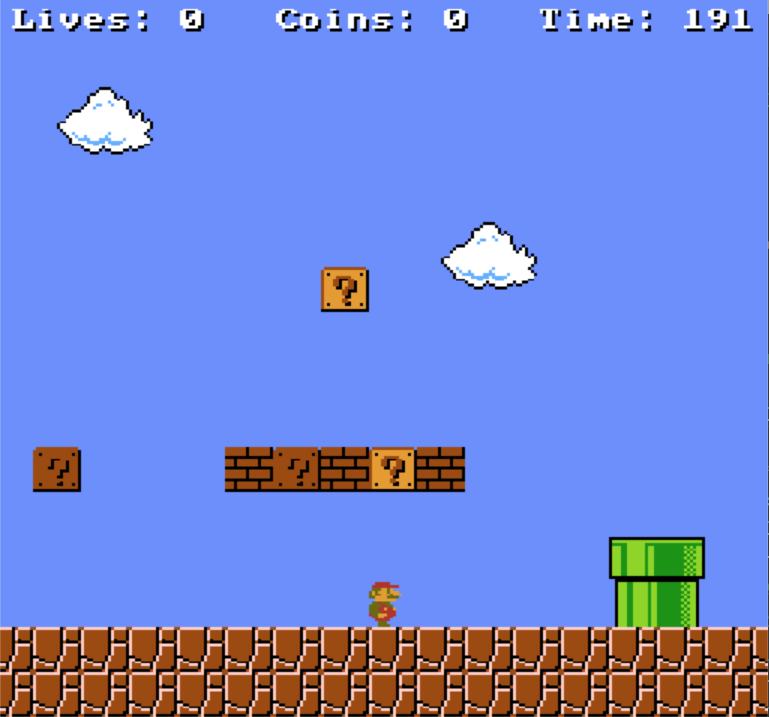
\includegraphics[width=0.48\linewidth]{Level1.png}
    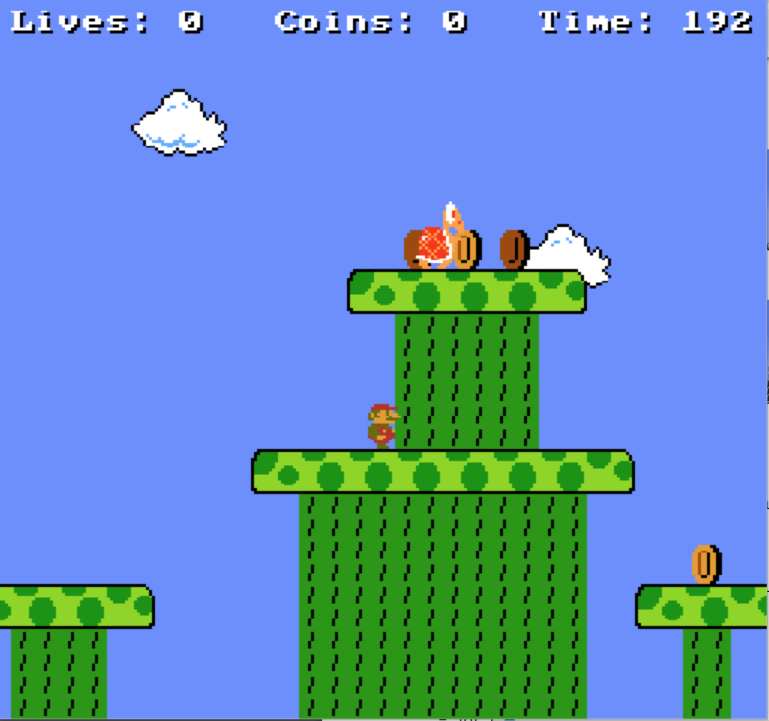
\includegraphics[width=0.48\linewidth]{Level3.png}
    \caption{These are the two scenes from the original Mario levels that we used to calculate KL Divergent.}
    \label{fig:KLDiv}
\end{figure}

\section{Visualization}\label{sec:Visualization}
For each of the 5 searching algorithms (CMA-ME, CMA-ES, MAP-ELITE, ISOLine-DD, random search), we made simulations 
on all 3 $BC$ settings discussed in Section \ref{sec:LevelEvaluation}. Figure \ref{fig:MarioGANBC} showed the elite 
maps of all 5 searching algorithms under the MarioGAN $BC$ setting.
\begin{figure*}[t!]
    \centering
    \begin{subfigure}[b]{.18\linewidth}
        \centering
        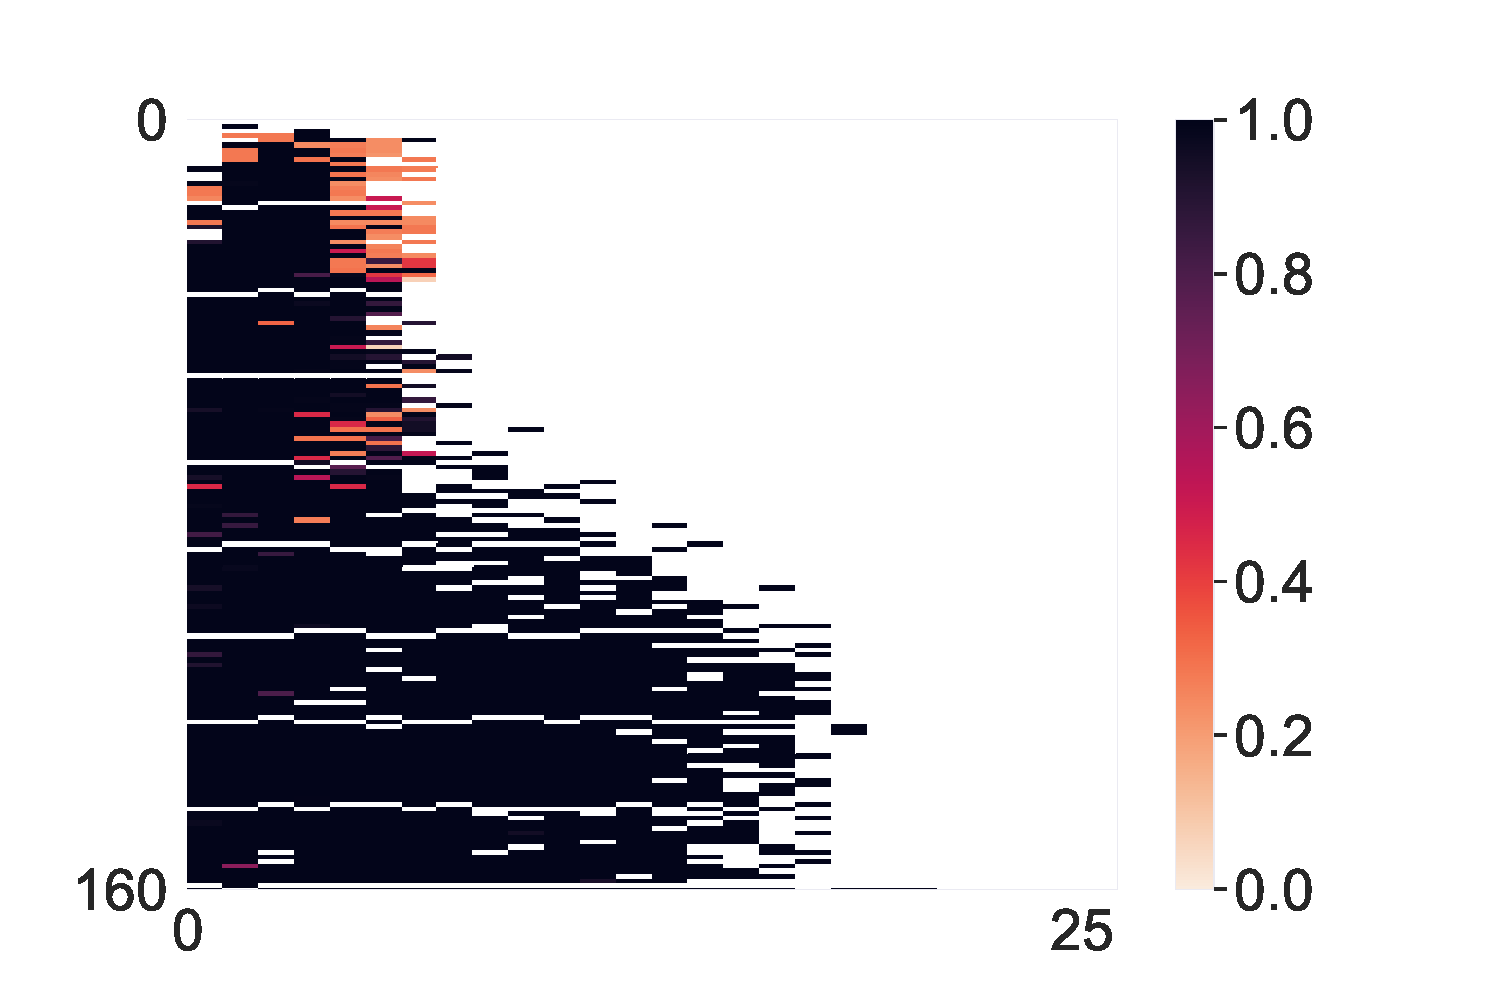
\includegraphics[width=\linewidth]{MarioGAN_map.pdf}
        CMA-ME
        \label{fig:CMAME_MarioGANBC}
    \end{subfigure}
    \begin{subfigure}[b]{.18\linewidth}
        \centering

        CMA-ES
        \label{fig:CMAES_MarioGANBC}
    \end{subfigure}
    \begin{subfigure}[b]{.18\linewidth}
        \centering
        
        MAP-ELITE
        \label{fig:MAPELITE_MarioGANBC}
    \end{subfigure}
    \begin{subfigure}[b]{.18\linewidth}
        \centering
        
        Random
        \label{fig:RANDOM_MarioGANBC}
    \end{subfigure}
    \begin{subfigure}[b]{.18\linewidth}
        \centering
        
        ISOLine-DD
        \label{fig:ISOLINEDD_MarioGANBC}
    \end{subfigure}
\caption{These were the elite maps of the 5 searching algorithms using MarioGAN $BC$ settings.}
\label{fig:MarioGANBC}
\end{figure*}
\end{document}